%===============================================================================
% $Id: ifacconf.tex 19 2011-10-27 09:32:13Z jpuente $  
% Template for IFAC meeting papers
% Copyright (c) 2007-2008 International Federation of Automatic Control
%===============================================================================
\documentclass{ifacconf}

\usepackage{graphicx}      % include this line if your document contains figures
\usepackage{natbib}        % required for bibliography
\usepackage{amsmath}
\usepackage{siunitx}
\usepackage{todonotes}

\usepackage{tikz}
\usetikzlibrary{arrows,automata,shapes}
\usepackage{xcolor}
\definecolor{green_node}{RGB}{188,213,190}
% \definecolor{purple_label}{RGB}{147,134,192}
% \definecolor{purple_label}{RGB}{194,188,213}
\definecolor{purple_label}{RGB}{157,153,173}

\usepackage{caption}
\usepackage{subcaption}
\usepackage{booktabs}
\usepackage{url}

%===============================================================================
\begin{document}
\begin{frontmatter}

\title{Ball in double hoop: Derivation of a mathematical model} 
% Title, preferably not more than 10 words.

\author{Martin Gurtner\quad} 


\end{frontmatter}
%===============================================================================

%-------------------------------- Model --------------------------------
\section{Modeling} % (fold)
\label{sec:model}
The system is cartooned in Fig.~\ref{fig:model_sketch} and the modes of the hybrid description are displayed in Fig.~\ref{fig:hybrid_modes}. The hybrid description has three modes: the ball rolls on the outer hoop (S1), the ball is in free fall (S2), and the ball rolls on the inner hoop (S3).

\begin{figure}[b]
\begin{center}
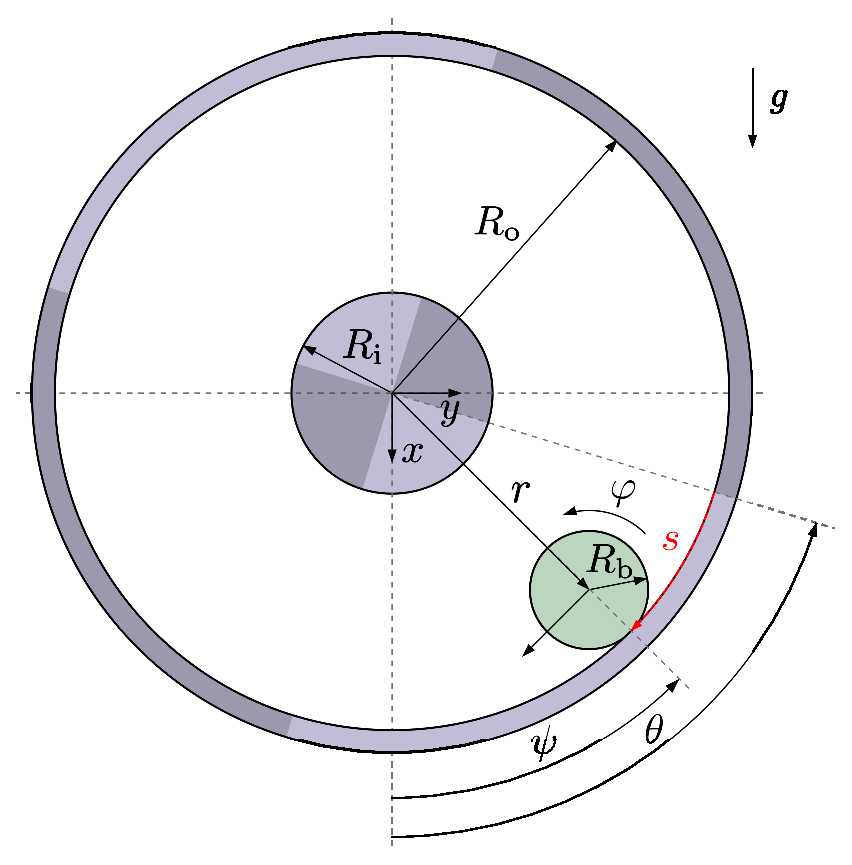
\includegraphics[width=5.5cm]{figs/sketchOfBallInAHoop3}    % The printed column width is 8.4 cm.
\caption{A sketch of the ball and hoop system.}
\label{fig:model_sketch}
\end{center}
\end{figure}

Before we delve into the derivation of equations of motion for each mode, let us devote a few words to coordinate systems in which we will describe the motion of the ball. Due to the rotational symmetry, polar coordinates are a natural choice for modes S1 and S3. In contrast, Cartesian coordinates are more suitable for the free-fall mode (S2) because then the equations of motion are linear. In fact, it turns out that the description of motion in S2 in polar coordinates is strongly nonlinear. Thus, from the implementation point of view (i.e. to increase numerical stability), one should use polar coordinates for modes S1 and S3 and Cartesian coordinates for S2. Nevertheless, transformations of the coordinates would make equations in this paper unnecessarily complicated, and thus we stick to polar coordinates for all three modes.

For simplicity, we will not state the time dependence explicitly. At first, we derive equations of motion for each mode and after that, we describe guards and reset maps for transitions between the modes.

\subsection{Outer hoop (S1)} % (fold)
\label{sub:outer_hoop}
A model of a ball rolling in a hoop was derived by~\cite{Wellstead1983Ball}. For reader's convenience---and because Wellstead made a small mistake in the derivation of the model---we rederive the model.

We use \textit{Euler-Lagrange equation} to derive the model. Let us choose angles $\psi$ and $\theta$ (see Fig.~\ref{fig:model_sketch}) as the generalized coordinates. We assume that the ball rolls without slipping. In addition, we assume that we can directly command the torque $\tau$ acting on the hoop.

The kinetic co-energy of the ball is
\begin{equation}
  T^\ast = \frac{1}{2} mv^2 + \frac{1}{2}I_\mathrm{b}(\dot{\varphi} + \dot{\theta})^2 + \frac{1}{2}I_\mathrm{h}\dot{\theta}^2,
\end{equation}
where $m$ is the mass of the ball, $I_\mathrm{b}$ is the moment of inertia of the ball, $I_\mathrm{h}$ is the moment of inertia of the hoop and $\varphi=\frac{s}{R_\mathrm{b}}=\frac{R_\mathrm{o}}{R_\mathrm{b}}(\theta-\psi)$. The translational velocity $v$ and the angular velocity $\dot{\varphi}$ of the ball can be expressed as follows
\begin{subequations}
\label{eq:kinematicConstraints}
  \begin{align}
  \label{eq:kinematicConstraints_vt}
    v &= -\left(R_\mathrm{o}-R_\mathrm{b}\right)\dot{\psi}, \\
  \label{eq:kinematicConstraints_phi}
    \dot{\varphi} &= \frac{R_\mathrm{o}}{R_\mathrm{b}}\left(\dot{\theta} - \dot{\psi}\right).  
  \end{align}
\end{subequations}
Thus, the kinetic energy expressed in the generalized coordinates is 
\begin{equation}
  T^\ast = \frac{1}{2} m\left(R_\mathrm{o}-R_\mathrm{b}\right)^2\dot{\psi}^2
  +
  \frac{1}{2}I_\mathrm{b}\left(\frac{R_\mathrm{o}+R_\mathrm{b}}{R_\mathrm{b}}\dot{\theta} - \frac{R_\mathrm{o}}{R_\mathrm{b}}\dot{\psi}\right)^2
  +
  \frac{1}{2}I_\mathrm{h}\dot{\theta}^2.
\end{equation}
Potential energy of the system is given by the potential energy of the ball and that is by
\begin{equation}
  V = -mg\left(R_\mathrm{o}-R_\mathrm{b}\right)\cos\psi
\end{equation}
and the system content modeling friction of the ball and hoop is
\begin{equation}
  D = \frac{1}{2}b_\mathrm{b}\dot{\varphi}^2 + \frac{1}{2}b_\mathrm{h}\dot{\theta}^2=\frac{1}{2}b_\mathrm{b}\frac{R_\mathrm{o}^2}{R_\mathrm{b}^2}\left(\dot{\theta} - \dot{\psi}\right)^2 + \frac{1}{2}b_\mathrm{h}\dot{\theta}^2.
\end{equation}

\begin{figure}[b]
  \center
  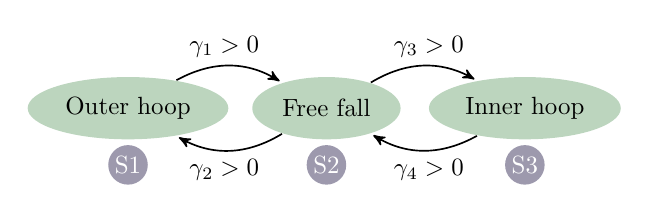
\begin{tikzpicture}[->,>=stealth',shorten >=1pt,auto,node distance=2.8cm,
                      semithick,scale=0.9, every node/.style={scale=0.9}]
    \tikzstyle{every state}=[fill=green_node,draw=none,text=black]
  
    \node[state,ellipse]    (A)                   {Outer hoop};
    \node[state,ellipse]    (B)[right of=A]       {Free fall};
    \node[state,ellipse]    (C)[right of=B]       {Inner hoop};
    \node[circle,inner sep=1.2pt,fill=purple_label]                   (A_label)[below of=A,node distance=0.8cm,text=white]       {S1};
    \node[circle,inner sep=1.2pt,fill=purple_label]                   (B_label)[below of=B,node distance=0.8cm,text=white]       {S2};
    \node[circle,inner sep=1.2pt,fill=purple_label]                   (C_label)[below of=C,node distance=0.8cm,text=white]       {S3};
  
    % \draw (A) -- (B);
    % \draw (B) -- (A);
    \path (A) edge  [bend left]       node[pos=0.45] {$\gamma_1>0$} (B)
        (B) edge  [bend left]        node[pos=0.55] {$\gamma_2>0$} (A)

        (B) edge  [bend left]       node[pos=0.55] {$\gamma_3>0$} (C)
        (C) edge  [bend left]        node[pos=0.45] {$\gamma_4>0$} (B);
          
  \end{tikzpicture}
  \caption{Modes of the hybrid description of the ball and hoop system.}
  \label{fig:hybrid_modes}
\end{figure}

Defining the Lagrangian $\mathcal{L}=T^\ast-V$, an equations of motion of the hoop and the ball, respectively, can be computed by Euler-Lagrange equation as
\begin{align}
  \frac{\mathrm{d}}{\mathrm{d}t}\left( \frac{\partial \mathcal{L}}{\partial \dot{\theta}} \right)
  -
  \frac{\partial \mathcal{L}}{\partial \theta}
  +
  \frac{\partial D}{\partial \dot{\theta}}
  =
  \tau \\
  \frac{\mathrm{d}}{\mathrm{d}t}\left( \frac{\partial \mathcal{L}}{\partial \dot{\psi}} \right)
  -
  \frac{\partial \mathcal{L}}{\partial \psi}
  +
  \frac{\partial D}{\partial \dot{\psi}}
  =
  0
\end{align}

which results in the following differential equation
\begin{equation}
  \bar{a}_\mathrm{o}\ddot{\psi} + \bar{b}_\mathrm{o}\dot{\psi} + \bar{c}_\mathrm{o}\sin\psi + \bar{d}_\mathrm{o}\dot{\theta} = \bar{e}_\mathrm{o}\ddot{\theta},
\end{equation}
with coefficients
\begin{subequations}
  \begin{align}
    \bar{a}_\mathrm{o} &= m \left(R_\mathrm{o}-R_\mathrm{b}\right)^2 + I \frac{R_\mathrm{o}^2}{R_\mathrm{b}^2}, \\
    \bar{b}_\mathrm{o} &= b  \frac{R_\mathrm{o}^2}{R_\mathrm{b}^2}, \\
    \bar{c}_\mathrm{o} &= m g \left(R_\mathrm{o}-R_\mathrm{b}\right), \\
    \bar{d}_\mathrm{o} &= -\bar{b}_\mathrm{o}, \\
    \bar{e}_\mathrm{o} &= I \frac{R_\mathrm{o}}{R_\mathrm{b}}\left( \frac{R_\mathrm{o}}{R_\mathrm{b}} + 1 \right).
  \end{align}
\end{subequations}
% subsection outer_hoop (end)

\subsection{Free fall (S2)} % (fold)
\label{sub:free_fall}
The motion of the center of the ball in free fall can be easily described in Cartesian coordinates because the only force acting on the ball is the gravitational force. Considering the Cartesian coordinate system shown in Fig.~\ref{fig:model_sketch}, we have 
\begin{equation}
  \ddot{x} = g
  \qquad \mathrm{and} \qquad
  \ddot{y} = 0.
\end{equation}
In order to get equations of motion in polar coordinates $(r,\psi)$ (see Fig.~\ref{fig:model_sketch}), we only need to transform the coordinates by relations $x=r\cos\psi$ and $y=r\sin\psi$. This way, we get
\begin{subequations}
  \begin{align}
    \ddot{r} &= r\dot{\psi}^2 + g\cos\psi, \\
    \ddot{\psi} &= -\frac{1}{r}\left(g\sin\psi + 2\dot{\psi}\dot{r}\right).
  \end{align}
\end{subequations}

To fully describe the state of the system during free fall of the ball we also need to describe evolution of $\varphi$; we assume that the angular velocity $\dot{\varphi}$ is constant during the free fall.

\begin{figure}
\begin{center}
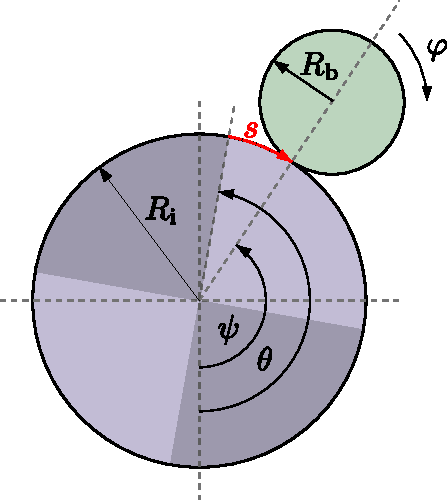
\includegraphics[width=3.7cm]{figs/inner}    % The printed column width is 8.4 cm.
\caption{A sketch of the ball rolling on the inner hoop.}
\label{fig:model_sketch_inner}
\end{center}
\end{figure}
% subsubsection transition_from_s2_to_s3 (end)
% subsection free_fall (end)

\subsection{Inner hoop (S3)} % (fold)
\label{sub:inner_hoop}
A sketch of the ball rolling on the inner hoop is shown in Fig.~\ref{fig:model_sketch_inner}. The equations of motion for the ball rolling on the inner hoop can be derived along similar lines as for the ball on the outer hoop. The only difference is that the effective rolling radius is $R_\mathrm{i}+R_\mathrm{b}$ instead of $R_\mathrm{o}-R_\mathrm{b}$ and angle $\varphi$ has the opposite orientation. Therefore, we skip the derivation and state directly the resulting equations of motion:
\begin{equation}
  \bar{a}_\mathrm{i}\ddot{\psi} + \bar{b}_\mathrm{i}\dot{\psi} + \bar{c}_\mathrm{i}\sin\psi + \bar{d}_\mathrm{i}\dot{\theta} = \bar{e}_\mathrm{i}\ddot{\theta},
\end{equation}
where
\begin{subequations}
  \begin{align}
    \bar{a}_\mathrm{i} &= m \left(R_\mathrm{i}+R_\mathrm{b}\right)^2 + I \frac{R_\mathrm{i}^2}{R_\mathrm{b}^2}, \\
    \bar{b}_\mathrm{i} &= b  \frac{R_\mathrm{i}^2}{R_\mathrm{b}^2}, \\
    \bar{c}_\mathrm{i} &= m g \left(R_\mathrm{i}+R_\mathrm{b}\right), \\
    \bar{d}_\mathrm{i} &= -\bar{b}_\mathrm{i}, \\
    \bar{e}_\mathrm{i} &= I \frac{R_\mathrm{i}}{R_\mathrm{b}}\left( \frac{R_\mathrm{i}}{R_\mathrm{b}} - 1 \right).
  \end{align}
\end{subequations}
% subsection inner_hoop (end)

\subsection{Transition between modes} % (fold)
\label{sub:transition_between_the_modes}

\subsubsection{Transition from S1 to S2} % (fold)
Mode S1 (outer hoop) is valid as long as the centripetal force $F_\mathrm{c}$ acting on the ball is larger then the normal component of the gravitational force $F_\mathrm{g}$ with respect to the hoop. Mathematically, it is valid if
\begin{equation}
\label{eq:mode1_validCondition}
  F_\mathrm{g}\cos\psi + F_\mathrm{c} = m g \cos\psi +  m\left( R_\mathrm{o} - R_\mathrm{b}\right)\dot{\psi}^2 > 0.
\end{equation}
If this condition does not hold, the ball drops of the hoop. It readily follows from~\eqref{eq:mode1_validCondition} that the guard for transition from S1 to S2 is
\begin{equation}
  \gamma_1  = - g \cos \psi -  \left( R_\mathrm{o} - R_\mathrm{b}\right)\dot{\psi}^2 > 0.
\end{equation}

The reset map for states $r$, $\dot{r}$, $\varphi$ and $\dot{\varphi}$ is
\begin{subequations}
\label{eq:resetMapS1_to_S2}
\begin{align}
  r^+            &= R_\mathrm{o}-R_\mathrm{b}, \\
  \dot{r}^+      &=   0, \\
  \varphi^+      &=   (\theta^- - \psi^-)\frac{R_\mathrm{o}}{R_\mathrm{b}}, \\
\label{eq:resetMapS1_to_S2_Dphi}  \dot{\varphi}^+  &= \frac{R_\mathrm{o}+R_\mathrm{b}}{R_\mathrm{b}}\dot{\theta} - \frac{R_\mathrm{o}}{R_\mathrm{b}}\dot{\psi}.
\end{align}
\end{subequations}
The first three relations are apparent. The last one is derived from the inertial angular velocity $(\dot{\varphi}^- + \dot{\theta}^-)$ of the ball and~\eqref{eq:kinematicConstraints_phi}. The remaining states transit to the mode S2 without any change, that is $\theta^+=\theta^-$, $\dot{\theta}^+=\dot{\theta}^-$, $\psi^+=\psi^-$ and $\dot{\psi}^+=\dot{\psi}^-$.

\subsubsection{Transition from S2 to S1} % (fold)
\label{ssub:transition_from_s2_to_s1}
This transition occurs when the ball hits the outer hoop. Thus the guard is
\begin{equation}
  \gamma_2 = r-R_\mathrm{o} + R_\mathrm{b}  > 0
\end{equation}
and the corresponding reset map for $\dot{\psi}$ is
\begin{equation}
\label{eq:resetMapS2_to_S1}
      \dot{\psi}^+ = \dot{\psi}^- + \dot{\psi}_\mathrm{rot}^-
\end{equation}
where $\dot{\psi}_\mathrm{rot}^-$ is derived from the angular velocity of the ball $\dot{\varphi}^-$ and can be computed from~\eqref{eq:kinematicConstraints_phi}:
\begin{equation}
      \dot{\psi}_\mathrm{rot}^- = \dot{\theta}^- - \frac{R_\mathrm{b}}{R_\mathrm{o}}\dot{\varphi}^-.
\end{equation}
The remaining states transit unchanged, that is $\theta^+=\theta^-$, $\dot{\theta}^+=\dot{\theta}^-$ and $\psi^+=\psi^-$.
% subsubsection transition_from_s2_to_s1 (end)

\subsubsection{Transition from S2 to S3} % (fold)
\label{ssub:transition_from_s2_to_s3}
Analogously to the previous case, the transit occurs when the ball hits the inner hoop and the guard is
\begin{equation}
  \gamma_3 = R_\mathrm{i} + R_\mathrm{b} - r > 0.
\end{equation}
The reset map is also almost the same; the only difference is that the angular velocity $\dot{\psi}_\mathrm{rot}^-$ here is computed as follows
\begin{equation}
\label{eq:resetMapS3_to_S2_Dpsi}
    \dot{\psi}_\mathrm{rot}^- = \dot{\theta}^- + \frac{R_\mathrm{b}}{R_\mathrm{i}}\dot{\varphi}^-.
\end{equation}

\subsubsection{Transition from S3 to S2} % (fold)
Similarly to the transition from the outer hoop to free fall, the transition from the inner hoop to free fall occurs when the centripetal force becomes larger then the normal component of the gravitational force with respect to the hoop, that is
$$
  \gamma_4 = g\cos{\psi} + \left(R_\mathrm{i} + R_\mathrm{b}\right)\dot{\psi}^2 > 0.
$$
and analogously to~\eqref{eq:resetMapS1_to_S2}, the reset map is
\begin{subequations}
\label{eq:resetMapS3_to_S2}
\begin{align}
  r^+            &= R_\mathrm{i}+R_\mathrm{b}, \\
  \dot{r}^+      &=   0, \\
  \varphi^+      &=   -(\theta^- - \psi^-)\frac{R_\mathrm{i}}{R_\mathrm{b}}, \\
  \dot{\varphi}^+  &=   -\left(\frac{R_\mathrm{i}-R_\mathrm{b}}{R_\mathrm{b}}\dot{\theta} - \frac{R_\mathrm{i}}{R_\mathrm{b}}\dot{\psi}\right),
\end{align}
\end{subequations}
with the remaining states $\theta$, $\dot{\theta}$, $\psi$ and $\dot{\psi}$ transiting unchanged.
% subsection transition_between_the_modes (end)
% section model (end)

\begin{align}
\label{eq:rollIt_OCP}
  \min_{u(t), x(t),T_\mathrm{f}} &\,\,\,  \int_{0}^{T_\mathrm{f}} u^2(t) \mathrm{d}t \\
 \nonumber       \text{subject to:}\,     &\,\,\, x(0) = x_0 \\
 \nonumber                          &\,\,\, x(T_\mathrm{f})  = x_\mathrm{f} \\
 \nonumber                          &\,\,\, 0 < T_\mathrm{f} < T_\mathrm{max} \\
 \nonumber                          &\,\,\, g\left(\mathbf{}{x}(t)\right) < 0 \\
 \nonumber                          &\,\,\, |u(t)| \leq u_\mathrm{max} \\
 \nonumber                          &\,\,\, \dot{\mathbf{x}}(t) = f(\mathbf{x}(t), u(t))
\end{align}


\begin{equation}
  x^\ast(t),\, u^\ast(t)
\end{equation}

\begin{align}
  \mathbf{A}(t) &= \frac{\partial f \left(\mathbf{x}(t), u(t)\right)}{\partial \mathbf{x}}\Big|_{\mathbf{x}(t) = \mathbf{x}^\ast(t), u(t)=u^\ast(t)} \\
  \mathbf{B}(t) &= \frac{\partial f \left(\mathbf{x}(t), u(t)\right)}{\partial u}\Big|_{\mathbf{x}(t) = \mathbf{x}^\ast(t), u(t)=u^\ast(t)}
\end{align}

$\delta\mathbf{x} = \mathbf{x} - \mathbf{x}^\ast$, $\delta u = u - u^\ast$
% section conclusion (end)

\bibliography{Remote}

\end{document}